%%
%% This is file `sample-sigconf.tex',
%% generated with the docstrip utility.
%%
%% The original source files were:
%%
%% samples.dtx  (with options: `sigconf')
%% 
%% IMPORTANT NOTICE:
%% 
%% For the copyright see the source file.
%% 
%% Any modified versions of this file must be renamed
%% with new filenames distinct from sample-sigconf.tex.
%% 
%% For distribution of the original source see the terms
%% for copying and modification in the file samples.dtx.
%% 
%% This generated file may be distributed as long as the
%% original source files, as listed above, are part of the
%% same distribution. (The sources need not necessarily be
%% in the same archive or directory.)
%%
%% The first command in your LaTeX source must be the \documentclass command.
\documentclass[sigconf]{acmart}
%% NOTE that a single column version may be required for 
%% submission and peer review. This can be done by changing
%% the \doucmentclass[...]{acmart} in this template to 
%% \documentclass[manuscript,screen]{acmart}
%% 
%% To ensure 100% compatibility, please check the white list of
%% approved LaTeX packages to be used with the Master Article Template at
%% https://www.acm.org/publications/taps/whitelist-of-latex-packages 
%% before creating your document. The white list page provides 
%% information on how to submit additional LaTeX packages for 
%% review and adoption.
%% Fonts used in the template cannot be substituted; margin 
%% adjustments are not allowed.
%%
%%
%% \BibTeX command to typeset BibTeX logo in the docs
\AtBeginDocument{%
  \providecommand\BibTeX{{%
    \normalfont B\kern-0.5em{\scshape i\kern-0.25em b}\kern-0.8em\TeX}}}

%% Rights management information.  This information is sent to you
%% when you complete the rights form.  These commands have SAMPLE
%% values in them; it is your responsibility as an author to replace
%% the commands and values with those provided to you when you
%% complete the rights form.
\setcopyright{acmcopyright}
\copyrightyear{2018}
\acmYear{2021}
\acmDOI{10.1145/1122445.1122456}

%% These commands are for a PROCEEDINGS abstract or paper.
\acmConference[Woodstock '18]{Woodstock '18: ACM Symposium on Neural
  Gaze Detection}{June 03--05, 2018}{Woodstock, NY}
\acmBooktitle{Woodstock '18: ACM Symposium on Neural Gaze Detection,
  June 03--05, 2018, Woodstock, NY}
\acmPrice{15.00}
\acmISBN{978-1-4503-XXXX-X/18/06}


%%
%% Submission ID.
%% Use this when submitting an article to a sponsored event. You'll
%% receive a unique submission ID from the organizers
%% of the event, and this ID should be used as the parameter to this command.
%%\acmSubmissionID{123-A56-BU3}

%%
%% The majority of ACM publications use numbered citations and
%% references.  The command \citestyle{authoryear} switches to the
%% "author year" style.
%%
%% If you are preparing content for an event
%% sponsored by ACM SIGGRAPH, you must use the "author year" style of
%% citations and references.
%% Uncommenting
%% the next command will enable that style.
%%\citestyle{acmauthoryear}

%%
%% end of the preamble, start of the body of the document source.
\begin{document}

%%
\title{Facial Expression Recognition for Cloud Robotics}

%%
%% The "author" command and its associated commands are used to define
%% the authors and their affiliations.
%% Of note is the shared affiliation of the first two authors, and the
%% "authornote" and "authornotemark" commands
%% used to denote shared contribution to the research.
\author{Charlie Maclean}
\affiliation{%
  \institution{University of Cambridge}
  \city{Cambridge}
  \country{United Kingdom}
}
\email{cm927@cam.ac.uk}


%%
%% By default, the full list of authors will be used in the page
%% headers. Often, this list is too long, and will overlap
%% other information printed in the page headers. This command allows
%% the author to define a more concise list
%% of authors' names for this purpose.
\renewcommand{\shortauthors}{Charlie Maclean}

\begin{abstract}

As social robots become widespread, it will be essential that they can
classify the emotions of humans around them, in order to interact in a
meaningful and helpful way. But limited hardware means they
may have to offload video data to the cloud (cloud robotics), reducing the resolution of the
content. This work focusses on evaluating the fitness of neural network models
for cloud computing, specifically the effect of changing spatial and temporal 
resolution on the
classification of emotion in video. We build different models to asses each
models performance when given lower resolution video. The results show that by
applying a CNN-LSTM model to a TODO 7-class problem, we can achieve 73\% accuracy on high resolution
video, and maintain 66\% accuracy with the lowest resolutions. To the best of
our knowledge this is the first work that investigates the effect of changing
both spatial and temporal resolution on video-based sentiment classification.

\end{abstract}


\keywords{Affective computing, robotics, cloud computing, emotions, arousal, valence, resolution.}

%%
%% This command processes the author and affiliation and title
%% information and builds the first part of the formatted document.
\maketitle

\section{Introduction}

\begin{figure}
  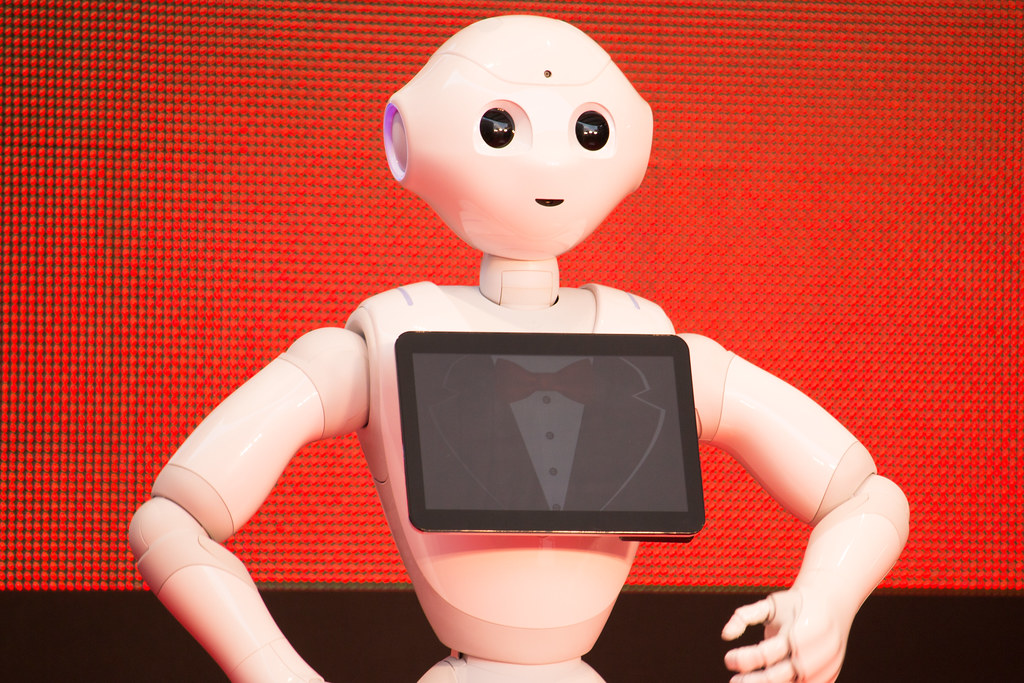
\includegraphics[width=\linewidth]{care-robot.jpg}
  \caption{Pepper by SoftBank Robotics, an example of a social robotic
  platform which has been trialled in care homes in the UK. Photograph by Dick
  Thomas, via creative commons.
  (\href{https://search.creativecommons.org/photos/e802da62-8b2f-4f10-9520-bb6c5a0e03db}{source})}
  \label{fig:pepper}
\end{figure}

Social robots are becoming increasingly widespread, with uses in a wide range
of locations, providing help in hospitals \cite{moxi}, care homes \cite{ElliQ}
and schools \cite{AV1}. These robots are frequently required to
interact meaningfully with humans, and in order to do so it is essential that
they are able to classify emotions to react accordingly. However, many social robotic
platforms lack the computational hardware required to perform classification
\cite{celiktutan18}.
Hence, it will likely become necessary to move to a cloud robotic framework,
where sensing data is offloaded to the cloud and processed there. Unreliable
network conditions mean we must be prepared for video data to enter the cloud
at reduced spatial and temporal resolutions. 

In past years, neural networks have become ubiquitous for classifying emotion,
due to their ability to learn pattern humans would be unable to program in.
However they can suffer from not being generalizable, especially if a network
is trained in one domain, then deployed in another. For example, a network
trained on high resolution data would be less effective at classifying low
resolution data. 

For classifying images, there is a large volume of work looking at using
convolutional neural networks (CNNs). When applied to an image, a CNN
convolves a filter with the pixel data, generating meaningful features. 
CNNs have found widespread use across various domains, including facial
recognition \cite{lawrence1997face} and object detection and classification
\cite{szegedy2014going}.
Several architectures have been proposed offering impressive ability to learn
features from video using 
purposes, for example the VGG16 network \cite{simonyan2014very} and the
ResNet50 network \cite{he2016deep}, both of which were able to achieve winning results in
the ImageNet object detection and classification challenge \cite{ILSVRC15}.

For classifying videos, it is often vital to take temporal data into account,
and as a result Recurrent Neural Networks (RNNs) \cite{rumelhart1985learning} are a good
choice. RNNs have some internal state, or memory, which they use to process
sequences, learning patterns that may vary over time. A very popular
architecture is Long Short Term Memory \cite{hochreiter1997long} {(LSTM), which make use of gates to
control the flow into and out of cells in the architecture. LSTMs have found
wide usage, across speech recognition \cite{graves2005framewise}, market prediction
\cite{islam2020foreign} and handwriting recognition \cite{graves2008unconstrained}.

In this work we create a couple of classifiers which are tested on video at a
variety of resolutions and frame-rates, in order to deduce which classifiers
may be useful for cloud robotics. The classifiers are tested on a 7-class
video dataset, and our results show that we can achieve an accuracy of X on

The rest of the paper is structured as follows: Section 2 gives an overview of
previous work on similar problems, Section 3 gives detail about the
methodology employed in the study. Then, Section 4 discusses the results
before Section 5 goes over future research directions. Finally, Section 6
concludes the paper with an overview of the findings. 

\section{Related Work}

In this section I give an overview of facial expression recognition
techniques, first for images, and then for videos, followed by a section 
on classifying data at reduced resolutions. 

\subsection{Facial Expression Recognition in Images}

Facial expressions have allowed humans to communicate their emotions amongst
each other for years. There has been a large volume of research into the
mechanisms which allow this non-verbal communication to happen. An early work
by P. Ekman and W.V. Friesen introduced the Facial Action Coding System
(FACS) \cite{friesen1978facial}, which described a list of facial action units
- regions which change as a person changes their expression. The work further describes
how a given facial expression could be described as a combination of action
units. Following this work, P. Ekman et al. detailed how a mapping can be made
between the facial action units and a person's emotions \cite{ekman1997face}. 
I will now detail the work that has been put into using machines to detect
emotions from photos, splitting the research into those that make use of deep
networks, and those before deep networks became widespread. 

Before the use of deep networks, there were two main approaches to sentiment
classification for images - rule-based methods, and appearance based methods.
First, the rule-based methods were centred around detecting facial action
units individually, and then piecing together the results from the facial
action unit recognizers to derive an overall emotion, for example in Y. Tian
et al.'s work \cite{tian2001recognizing}. These techniques
suffered as recognizing an individual action unit is not an easy task. In the
alternative approach, appearance based methods, some features are extracted
from the overall face, and then those features are passed through a machine
learning classifier. For example, M.S. Bartlett et al. found that they could
achieve good results by extracting features using Gabor filters, followed by a
Support Vector Machine (SVM) \cite{bartlett2005recognizing}. Additionally, J.
Whitehall and C. Omlin showed that comparable results could be obtained in
significantly quicker time by instead using Haar wavelets to obtain features
before passing through a SVM \cite{whitehill2006haar}. 

In previous techniques, processing of emotions had been split into learning
features, selecting features and then using a classifier to learn the
patterns. The downside of taking that approach is that the first layers do not
get feedback from the latter layers. Deep learning aims to solve that, by
integrating the feature finding, selection and classification into one deep
network that can be trained at once. One of the early papers making use of
this technique was by P. Liu et al. \cite{liu2014facial}, who suggested using
a Boosted Deep Belief Network. This network consisted of several deep networks
learning features, and some of these networks get boosted based on their
performance. Finally, in \cite{liu2016facial}, Liu et al. introduced CNNs to the 
problem, with their CNN Ensemble network. The network consisted of three 
different convolutional networks, which proved to achieve better results than
a single CNN.

\subsection{Facial Expression Recognition in Videos}

When classifying emotion in videos, there is additional information that can
be extracted by accounting for the way the face changes over time. There are
several papers which attempt to do this, which I will now go over, beginning
with aggregation techniques. Aggregation techniques classify each frame within
a video, and then combine the results with some sort of aggregator. In
\cite{kahou2016emonets} and \cite{kahou2013combining}, S. Kahou et al. split
the video into 10 sections, and within each section aggregate the frame
predictions with an average. They go on to use a SVM to classify using all 10
aggregate predictions. An alternative method was introduced in 
\cite{liu2014combining} where
M. Liu et al. showed that features from individual frames could be mapped to 
linear subspaces, covariance matrices or Gaussian distributions, allowing
these to be passed to a support vector machine.

An alternative approach focussed on attempts to classify the level of
emotional intensity present in an individual frame - the idea being that you
could derive the emotion of a video base on the strongest emotions present. 
In \cite{zhao2016peak} X. Zhao et al. propose a network which minimizes the differences
between an emotion at low intensity and the same emotion at high intensity, as
a way to get better classification of low intensity emotion. The downside of
their technique was that it required a training set consisting of pairs of the
same emotions at different intensities. To address this, 
in \cite{chen2018deep} J. Chen et al. used unsupervised clustering and a semisupervised 
SVM to detect peak and neutral frames in a large dataset.

Finally, deep spatio-temporal networks were introduced which use sequences of
frames as inputs to the networks, in the hopes that we can learn more
information from the temporal dynamics of the images. C3Ds
\cite{tran2015learning} are the natural generalization of a CNN to 3
dimensions - instead of convolving an image with a 2D kernel, we convolve a
sequence of frames with a 3D kernel. These 3D techniques have been bought to
video emotion recognition, for example by X. Ouyang in \cite{ouyang2017audio}.
An alternative approach was taken in \cite{kim2017multi} where D. Kim et al.
tracked facial landmarks to generate trajectories which were used as features.
Finally, a common approach is to use a CNN to learn spatial features of an
image followed by a LSTM to learn the temporal features of the overall video, as in
\cite{kim2017multiobjective}.

\subsection{Reduced resolution classification}

There have been a couple of studies looking at how to cope when the face that
needs to be classified is at a low resolution. Firstly, Y. Tian
\cite{tian2004evaluation} looked at how low spatial resolution would affect
three steps in a facial expression analysis pipeline: face acquisition,
facial data extraction and finally expression recognition. 


\section{Facial Expression Recognition}
\subsection{Images}



\section{Methodology}

\subsection{Transfer Learning}

In order to efficiently train on 

\section{Future Work}
%%
%% Future work:
%% - Multimodal analysis
%% - Testing on in the wild datasets
%% - 

\section{Conclusion}


%%
%% The next two lines define the bibliography style to be used, and
%% the bibliography file.
\bibliographystyle{ACM-Reference-Format}
\bibliography{writeup}

%%
%% If your work has an appendix, this is the place to put it.

\end{document}
\endinput
%%
%% End of file `sample-sigconf.tex'.
